% Template file for an a0 portrait poster.
% Written by Graeme, 2001-03 based on his SOC poster.
%
% See discussion and documentation at
% <http://www.astro.gla.ac.uk/users/norman/docs/posters/> 
%
%%%%%%%%%%%%%%%%%%%%%%%%%%%%%%%%%%%%%%%%
% Modified by Jozef Dobo\v{s} (c) 2011 % 
%%%%%%%%%%%%%%%%%%%%%%%%%%%%%%%%%%%%%%%%

\documentclass[a0,portrait]{a0poster}
% You might find the 'draft' option to a0 poster useful if you have
% lots of graphics, because they can take some time to process and
% display. (\documentclass[a0,draft]{a0poster})

\pagestyle{empty}
\setcounter{secnumdepth}{0}
\usepackage[absolute,
					%showboxes
					]{textpos}
\usepackage{txfonts}
\usepackage{wrapfig,times}
\usepackage[scaled]{helvet}
\usepackage{graphicx}
\usepackage{forloop}
\usepackage[margin=0cm]{geometry}
\usepackage{wasysym}
\usepackage{enumitem}
\usepackage{tipa}
\usepackage{tikz}
\usetikzlibrary{backgrounds}
\usepackage{cleveref}


%%%%%%%%%%
% Colors %
%%%%%%%%%%
\usepackage{color}
\definecolor{TitleColor}{rgb}{1,1,1} % white
\definecolor{BannerOneColor}{rgb}{0,0,0} % pitch black
\definecolor{BannerTwoColor}{rgb}{0.93,0.08,0.31} % pinky red
\definecolor{BannerThreeColor}{rgb}{0,0.27,0.48} % dark blue
\definecolor{BannerFourColor}{rgb}{0.33,0.19,0.098} % brown
\definecolor{BannerSixColor}{rgb}{0,0.27,0.42} % dark blue
\definecolor{BannerSevenColor}{rgb}{0.62,0.77,0.86} % sky blue
\definecolor{BannerEightColor}{rgb}{0.35,0.33,0.01} % military green
\definecolor{BannerNineColor}{rgb}{0.85,0.86,0.34} % lime green
\definecolor{BannerTenColor}{rgb}{0,0.66,0.80} % strong blue
\definecolor{BannerElevenColor}{rgb}{0.46,0,0.20} % maroon
\definecolor{BannerTwelveColor}{rgb}{0.37,0.32,0.44} % dark washed violet
\definecolor{BannerThirteenColor}{rgb}{0.79,0.84,0.65} % light washed green
\definecolor{BannerFourteenColor}{rgb}{0.57,0.64,0.27} % dark washed green
\definecolor{BannerFifteenColor}{rgb}{0.92,0.91,0.88} % unusable washed 
\definecolor{BannerSixteenColor}{rgb}{0.94,0.36,0.14} % strong orange
\definecolor{BannerSeventeenColor}{rgb}{0.97,0.61,0.19} % orange
\definecolor{BannerEighteenColor}{rgb}{0.99,0.76,0.11} % mustard yellow
\definecolor{BannerNineteenColor}{rgb}{0.79,0.76,0.73} % light gray-ish
\definecolor{BannerTwentyColor}{rgb}{0.63,0.58,0.54} % dark gray-ish

\def\bannercolor{BannerSixColor}

%%%%%%%%%%%%%%%%%%%%%%%%%%%%%%%%%%%%%%%%%%%%%%%%%%%%%%
% Only change here to affect all headings            %
\newcommand{\headingcolor}{\color{BannerSixColor}} 
\newcommand{\titlecolor}{\color{TitleColor}}
%\newcommand{\banner}{\includegraphics[width=\linewidth]{banners/darkblue.pdf}}
\newcommand{\banner}{\LARGE \tikz{\path[draw=\bannercolor,fill=\bannercolor] (0,0) rectangle (\linewidth,2.25em);}}
\def\Highlight#1{{\sffamily \headingcolor #1}}
%%%%%%%%%%%%%%%%%%%%%%%%%%%%%%%%%%%%%%%%%%%%%%%%%%%%%%

% see documentation for a0poster class for the size options here
\let\Textsize\Large
\def\Head#1{\noindent\hbox to \hsize{\hfil{\LARGE \headingcolor #1}}\bigskip}
\def\LHead#1{\noindent{\sffamily \LARGE \headingcolor #1}\smallskip}
\def\Authors#1{\noindent{\sffamily \LARGE #1}\smallskip}
\def\Subhead#1{\noindent{\large \headingcolor #1}}
\def\Title#1{\noindent{\sffamily \VeryHuge \titlecolor #1}}

\setlist[itemize,1]{topsep=0pt, itemindent=1cm, labelsep=1cm, label={{\headingcolor $\bullet$}}}
\setlist[itemize,2]{topsep=0pt, itemindent=2cm, labelsep=1cm, label={{\headingcolor $\triangleright$}}}
%\setitemize{topsep=0pt}

% Set up the grid
%
% Note that [0cm,0cm] is the margin round the edge of the page --
% it is _not_ the grid size. That is always defined as 
% PAGE_WIDTH/HGRID and PAGE_HEIGHT/VGRID. In this case we use
% 25 x 25. This gives us three wide columns for text (7 grid
% spacings) and four narrow columns (1 each) at each side of these 
% text columns
%
% Note however that texblocks can be positioned fractionally as well,
% so really any convenient grid size can be used.
%

% [margin, margin]{rows}{cols}
\TPGrid[0cm,0cm]{17}{25}  % 1 - 7 - 1 - 7 - 1 Columns


% Mess with these as you like
\parindent=0pt
%\parindent=1cm
\parskip=0.5\baselineskip
\linespread{1.2}

% abbreviations
\newcommand{\ddd}{\,\mathrm{d}}

\begin{document}

% Understanding textblocks is the key to being able to do a poster in
% LaTeX. In
%
%    \begin{textblock}{width}(x,y)
%    ...
%    \end{textblock}
%
% the first argument gives the block width in units of the grid
% cells specified above in \TPGrid; the second gives the (x,y)
% position on the grid, with the y axis pointing down.

%%%%%%%%%%%%%%
% Top Banner %
%%%%%%%%%%%%%%


%\begin{tikzpicture}[remember picture, overlay]
%\begin{pgfonlayer}{background}
%  \path[draw=BannerTwelveColor,fill=BannerTwelveColor] (0,0) rectangle (\paperwidth,9cm);
%\end{pgfonlayer}
%\end{tikzpicture}

 %if you change this part, you can get matching color for headings
 %in Colors section above
\begin{textblock}{17}(0,0) {
%\includegraphics[width=\paperwidth]{banners/darkblue.pdf}
%\includegraphics[width=\paperwidth]{banners/purple.pdf}
\VeryHuge
\tikz{\path[draw=\bannercolor,fill=\bannercolor] (0,0) rectangle (\paperwidth,3.5em);}
} \end{textblock}




%%%%%%%%%
% Title %
%%%%%%%%%
%TODO MAKE TITLE BANNER BIGGER/LESS CRAMPED
\begin{textblock}{10}(1,0.5)
{\color{TitleColor}
\Title{A CAPT tool for training and research on lexical stress errors in German}\\

%\Authors{Anjana Vakil}, {\sffamily \Large Computational Linguistics}\\
%\textbf{\large \texttt{anjanav@coli.uni-saarland.de}}
}
\end{textblock}

\begin{textblock}{4}(12,0.25)    
\begin{flushright}
%\resizebox{1.5\TPHorizModule}{!}{

\includegraphics[width=1.3\TPHorizModule]{../../../img/new-owl-white.png}
%
\includegraphics{images/saarland_university_white.png}
%
\includegraphics{images/uds-logo-text-white.png}
\end{flushright}
\end{textblock}

\begin{textblock}{4}(10.5,0.5){
\color{TitleColor}
\begin{flushright}
\Authors{Anjana Vakil}\\
{\sffamily \Large Computational Linguistics}\\%, Saarland University}\\
{\sffamily \Large Saarland University}\\
\textbf{\large \texttt{anjanav@coli.uni-saarland.de}}
\end{flushright}
}
\end{textblock}

%\begin{textblock}{5}(1,2){
%\headingcolor
%\Authors{Anjana Vakil}\\
%{\sffamily \Large Computational Linguistics, Saarland University}\\%, U. Saarland}\\
%\textbf{\large \texttt{anjanav@coli.uni-saarland.de}}
%}
%\end{textblock}


%\section{Introduction}

% An example text block, to get you started!
\begin{textblock}{7}(1, 2.75) {
\banner
} \end{textblock}
\begin{textblock}{6.75}(1.25,3){
  \LHead{\titlecolor Overview}}
 \end{textblock}
 \begin{textblock}{7}(1, 3.75)
  \Textsize
This poster presents the prototype Computer-Assisted Pronunciation Training (CAPT) tool \Highlight{de-stress}: the German (\Highlight{de}) \Highlight{S}ystem for \Highlight{T}raining and \Highlight{R}esearch on \Highlight{E}rrors in \Highlight{S}econd-language \Highlight{S}tress [1].

\Highlight{de-stress} targets lexical stress errors by non-native (L2) German speakers with French as their native language (L1). Its modular design incorporates various methods for diagnosing and presenting feedback on these errors. Both instructional and research applications have motivated its development:

\begin{itemize}
\item{Learners can interact with the system independently (i.e. without assistance from human instructor)}
\item{Teachers can create bespoke exercises for students}
\item{Researchers can study effects of various diagnois/feedback types}
\item{Tool could become useful component of intelligent CAPT system (see \cref{fig:hourglass-ITS})}
\end{itemize}



%\Highlight{Context:} M.Sc. thesis, related to ongoing Franco-German project\\ \textit{Individualized Feedback for Computer-Assisted Spoken Language\\ Learning} (IFCASL) [3].
%% at University of Saarland (Saarbr{\"u}cken, Germany) and LORIA (Nancy, France).

\vspace{1em}

	\begin{figure}
	\centering
	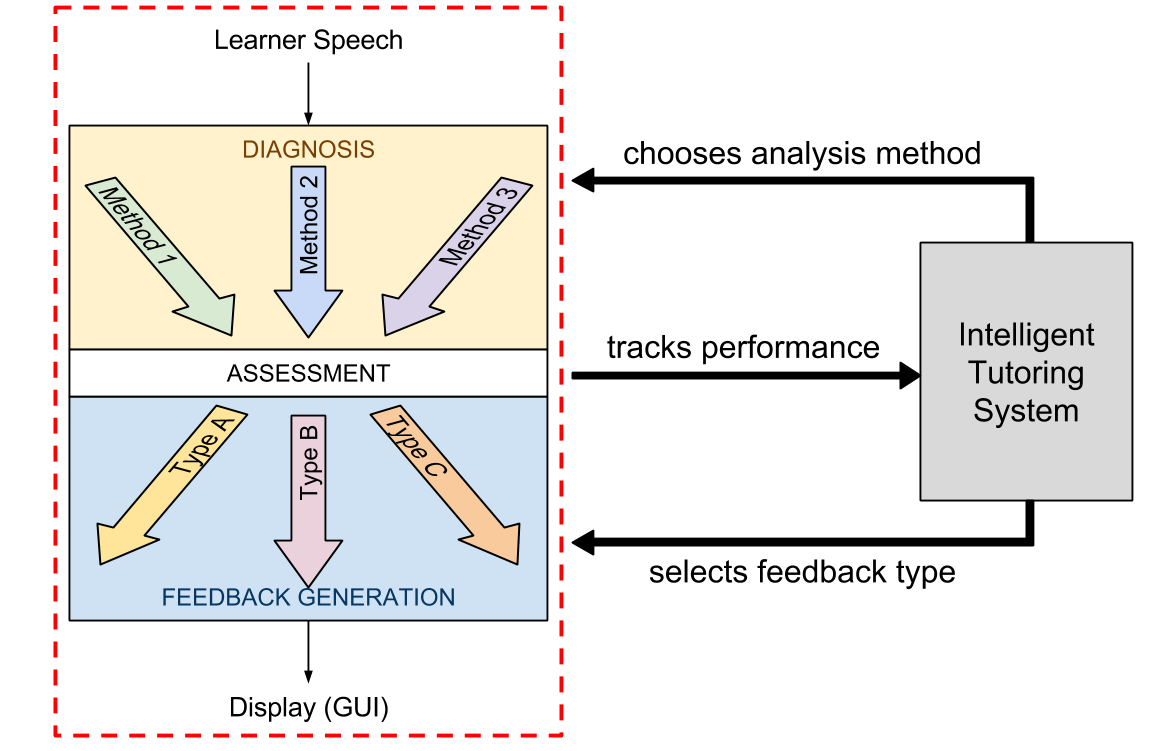
\includegraphics[width=\textwidth]{../../../colloquium/hourglass-colloq-full}
	\caption{Conceptual diagram of \Highlight{de-stress} (demarcated by dashed line) and its possible function in the context of an Intelligent Tutoring System (ITS).}
	\label{fig:hourglass-ITS}
	\end{figure}
 
\end{textblock}


%\section{Training tool}

\begin{textblock}{7}(1, 15.75) {
\banner
} \end{textblock}
\begin{textblock}{6.75}(1.25,16){
  \LHead{\titlecolor A training tool for German learners}}
 \end{textblock}
 \begin{textblock}{7}(1, 16.75)
\Textsize


	\begin{center}
	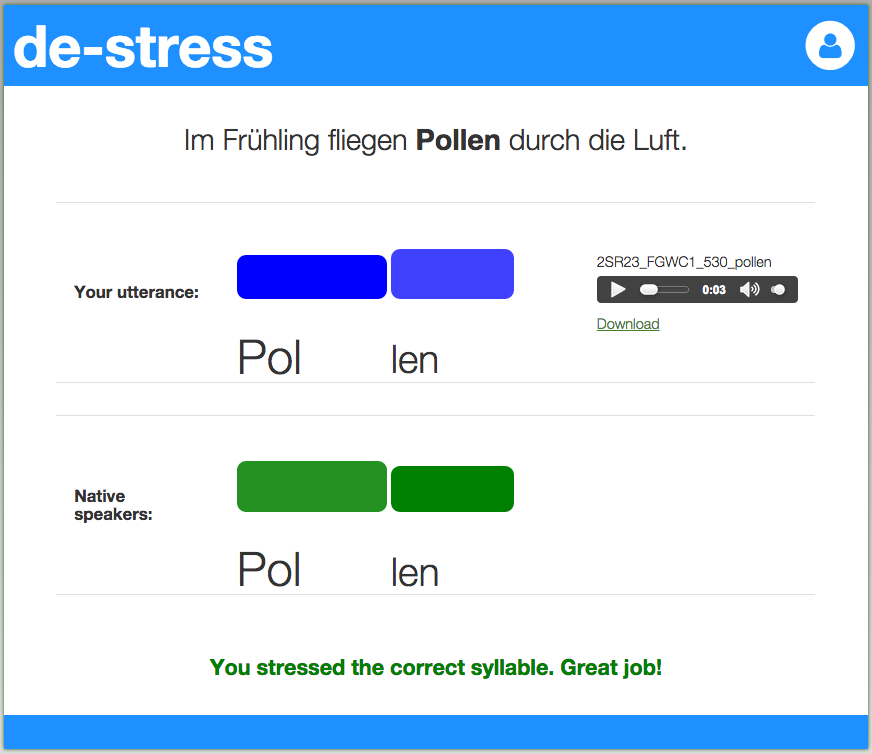
\includegraphics[width=.7\textwidth]{../../../img/screenshots/StudentInterface-userIcon}
	\end{center}

\end{textblock}


%\section{Teaching and research tool}

\begin{textblock}{7}(9, 2.75) {
\banner
} \end{textblock}
\begin{textblock}{6.75}(9.25,3){
  \LHead{\titlecolor A tool for teachers and researchers}}
 \end{textblock}
 \begin{textblock}{7}(9, 3.75)
  \Textsize
  
  An administrative interface allows language teachers or CAPT researchers to combine the available diagnostic and feedback method(s) to create new exercises for learners. 
  
%  \begin{itemize}
%  \item{Teachers can create exercises targeted to students' needs (learning style, etc.)}
%  \item{Researchers can study impact of various diagnosis/feedback configurations on factors impacting CAPT system success, e.g.
%  \begin{itemize}
%  \item{learning outcomes}
%  \item{user engagement/satisfaction}
%  \end{itemize}
%  }
%  \end{itemize}
 
	\begin{center}
	\fcolorbox{gray!50}{white}{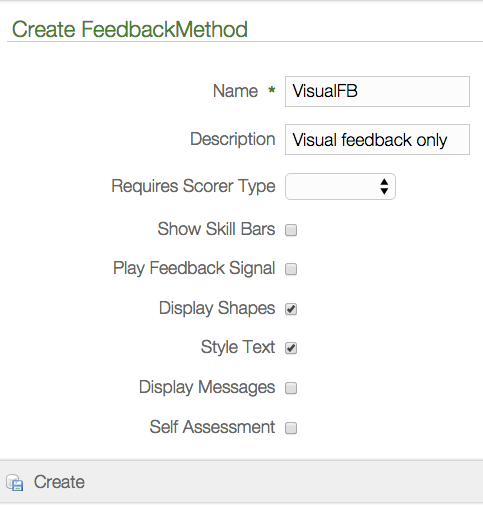
\includegraphics[width=.7\textwidth]{../FeedbackMethod}}
	\end{center}	  
  
  
\end{textblock}


%\begin{textblock}{7}(9, 8.5) {
%\banner
%} \end{textblock}
%\begin{textblock}{6.75}(9.25,8.75){
%  \LHead{\titlecolor A teaching and research tool}}
% \end{textblock}
% \begin{textblock}{7}(9, 9.5)
%  \Textsize
% 
%\end{textblock}



\%section{Conclusion}

% Another text block in the bottom right.
\begin{textblock}{7}(9,13){
\banner
} \end{textblock}
\begin{textblock}{6.75}(9.25,13.25){
  \LHead{\titlecolor Conclusion and future directions}
   } \end{textblock}
 \begin{textblock}{7}(9, 14)
  \Textsize
  
%  Both instructional and research applications have thus motivated the development of \Highlight{de-stress}.
%Unlike with some existing tools for diagnosis and feedback on pronunciation errors, learners can interact with the tool and interpret its feedback independently, i.e. without the assistance of a human instructor at their side.
%At the same time, researchers can use this modular system to study the impact of various assessment and feedback types on learner outcomes, user engagement, and other factors impacting the success of a CAPT system. 
%%
%Once more is known about which diagnosis/feedback types should be delivered to which learners in which situations, this tool could become a useful component of a fully-fledged intelligent CAPT system, in which 
%%learner models and other intelligent components
%models of relevant aspects of the learning context (e.g. the student's skill level, progress, or personal preferences; the current learning objective or position in a sequence of exercises; etc.)
%are used to automatically decide which modules of the tool to activate, as \cref{fig:hourglass-ITS} illustrates.
  
  
  
\end{textblock}



%\section{References}

\begin{textblock}{7}(9,22.5){
\banner
} \end{textblock}
\begin{textblock}{6.75}(9.25,22.75){
  \LHead{\titlecolor References}
   } \end{textblock}
 \begin{textblock}{7}(9, 23.3)
%  \Textsize
%  
%  
%\end{textblock}
%
%
%\begin{textblock}{15}(1,23)
%{\Large
%\tikz{\path[draw=\bannercolor,fill=\bannercolor] (0,0) rectangle (\linewidth,2em);}}
%\end{textblock}
%\begin{textblock}{14.75}(1.15,23.15)
%\LHead{\Large \titlecolor References}
%\end{textblock}
%\begin{textblock}{15}(1,23.55)

\begin{enumerate}[label={[\arabic*]}, leftmargin=34pt, topsep=0pt]

\item{A. S. Vakil, "de-stress," \texttt{http://github.com/vakila/de-stress}.}

\item{LORIA Speech Team, "JSnoori," \texttt{http://jsnoori.loria.fr}.}

\item{A. S. Vakil and J. Trouvain, "Automatic classification of lexical stress errors for German CAPT," in \textit{SLaTE}, 2015.}

%\item{Trouvain, J., et al. 2013. ``Designing a bilingual speech corpus for French and German language learners''. \textit{Proc. Corpus et Outils en Linguistique, Langues et Parole}, Strasbourg, pp. 32-34.}
\end{enumerate}

\end{textblock}

%\begin{textblock}{15}(1,23.25)
%\LHead{\Large \headingcolor References}
%\begin{enumerate}[label={[\arabic*]}, leftmargin=34pt, topsep=0pt]
%\item{Bonneau, A. and V. Colotte. 2011. “Automatic Feedback for L2 Prosody Learning”. In \textit{Speech and Language Technologies}. Ivo Ipsic, ed. InTech.}
%
%\item{Hirschfeld, U. 1994. \textit{Untersuchungen zur phonetischen Verst{\"a}ndlichkeit Deutschlernender.} Forum Phoneticum, 57.}
%
%\item{Trouvain, J., et al. 2013. ``Designing a bilingual speech corpus for French and German language learners''. \textit{Proc. Corpus et Outils en Linguistique, Langues et Parole}, Strasbourg, pp. 32-34.}
%\end{enumerate}
%
%\end{textblock}


% If you want to add a figure do something like this:

%\begin{textblock}{3}(1,15)
%  \begin{center}
%  \resizebox{3\TPHorizModule}{!}{\includegraphics{images/group-logo.pdf}}
%\\{\bfseries Figure 5:} caption
%  \end{center}
%\end{textblock}



% Place the group logo at the bottom left - visually this balances
% well with the University logo at the top right. 
%\begin{textblock}{4}(1,23)    
%%\resizebox{1.5\TPHorizModule}{!}{
%
\includegraphics{images/uds-logo-text.png}
%%}
%\end{textblock}



\end{document}

